\section{Afstand}
\label{DatabehandlingRAfstand}
%
I dette afsnit analyseres resultaterne med udgangspunkt i de tre forskellige afstanden robotten havde til testpersonerne i testen. De forskellige afstande fremgår af \autoref{tab:RDistance}, hvor antallet af testpersoner ligeledes er opgivet. 

Det undersøges, hvordan robottens afstand påvirker de rejsendes oplevelse af robotten ved at undersøge, hvordan resultaterne ændrer sig afhængigt af de tre forskellige afstande. Det er et \textit{Between-subject} design, da hver testperson kun har oplevet robotten i én af afstandende og svaret ud fra denne.
%
\begin{table}[H]
\centering
\begin{tabular}{c|c}
Afstand & Antal testpersoner \\ \hline
Tæt på (1) & 7    \\ \hline
Tilpas (2) & 28    \\ \hline
Langt fra (3) & 8     \\ 
\end{tabular}
\caption{Oversigt over antallet af testpersoner til hver af de tre afstande robotten havde.}
\label{tab:RDistance}
\end{table}
\noindent
%
Ud fra \textit{Scree}-plottet på \autoref{fig:Distance-Scree} fremgår det at cirka 80 \& af variansen kan forklares ud fra den første \textit{Principal Component} (PC) og 100 \% af variansen kan forklares ud fra to PCs. 
%
\begin{figure}[H]
\centering
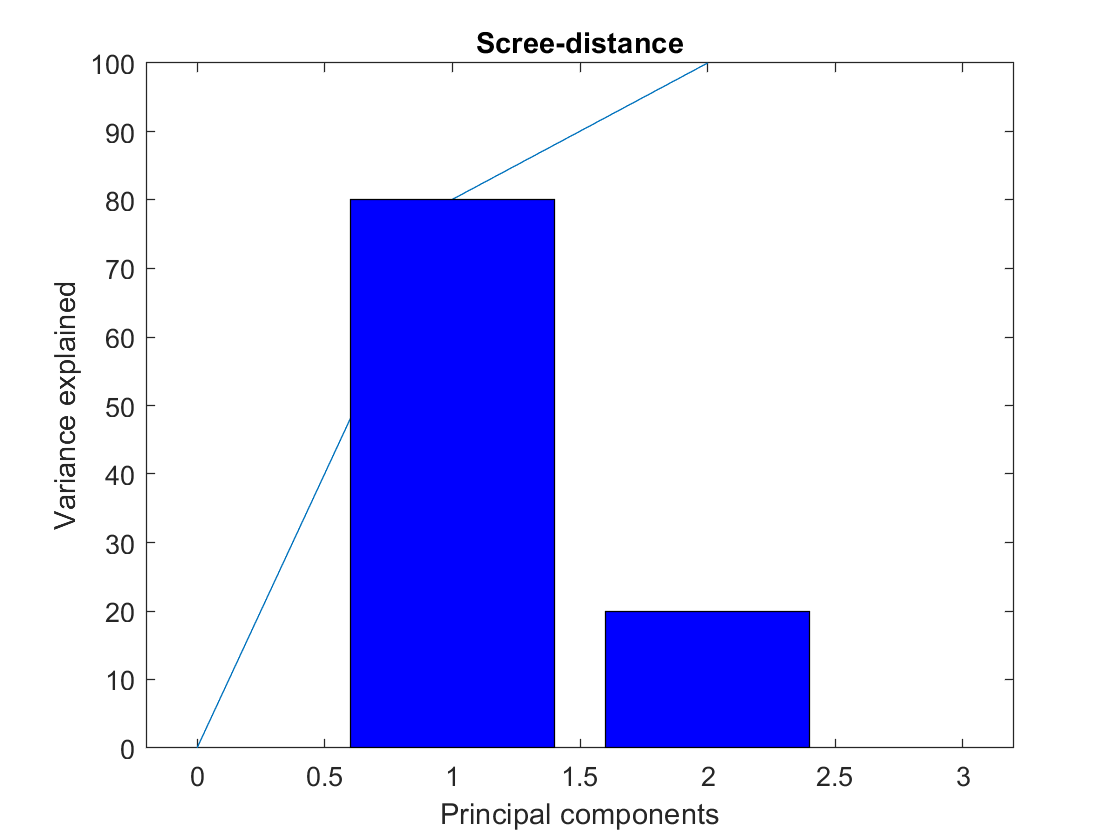
\includegraphics[width=\textwidth]{Figure/DatabehandlingSkalaer/PCAfigures/Distance-Scree.png}
\caption{\textit{Scree}-plot, hvorpå sammenhængen mellem antallet af \textit{Principal Components} og \textit{Variance Explained [\%]} fremgår.}
\label{fig:Distance-Scree}
\end{figure}
\noindent
%
Ud fra \textit{Score}-plottet på \autoref{fig:Distance-Score} fremgår det, at der generelt er en del spredning mellem resultaterne ud fra de tre forskellige afstande, hvilket foreskriver at det de tre afstanden ikke umiddelbart har ens karakteristikas. 
%
\begin{figure}[H]
\centering
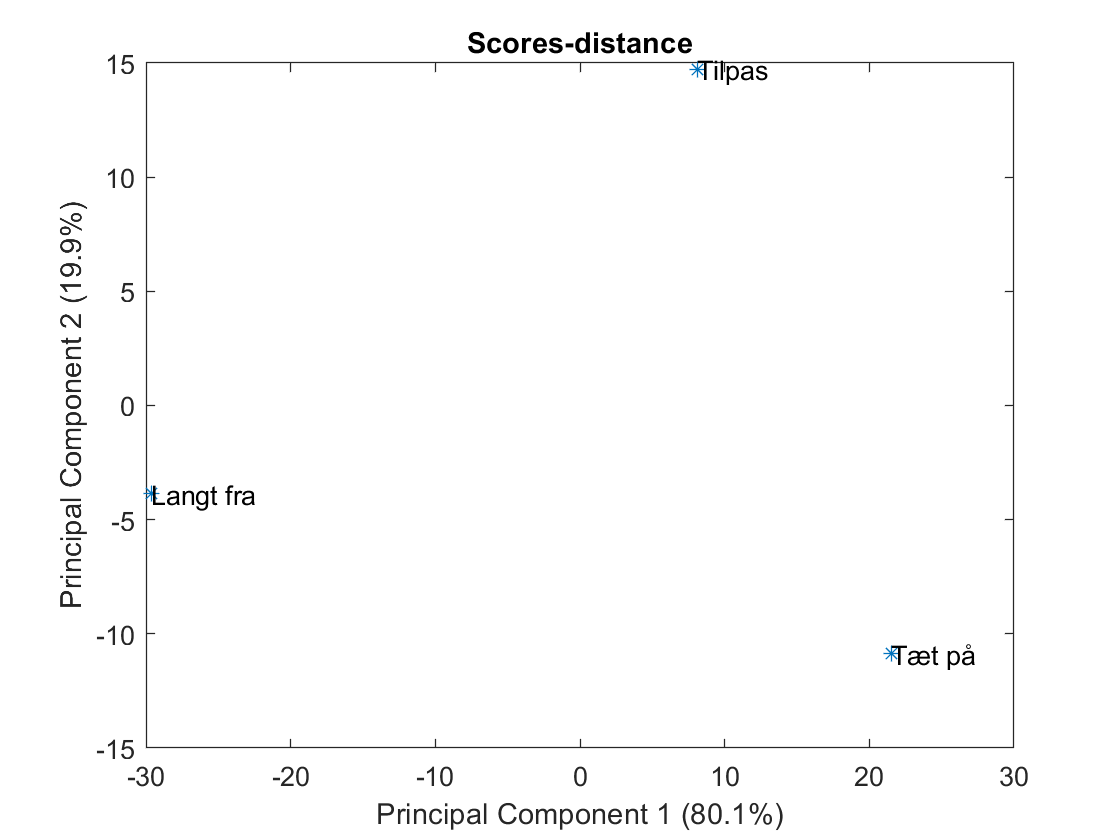
\includegraphics[width=\textwidth]{Figure/DatabehandlingSkalaer/PCAfigures/Distance-Scores}
\caption{\textit{Score}-plot for PC1 og PC2 i forhold til de tre afstande robotten holder til testpersonerne.}
\label{fig:Distance-Score}
\end{figure}
\noindent
%
Ud fra \textit{Bi}-plottet på \autoref{fig:Distance-Biplot}, hvorpå \textit{loadings} og \textit{scores} for hver parameter er præsenteret, fremgår det at SQ1, omhandlende skærmens reaktion, og SQ15, omhandlende hvor overraskede testpersonerne blev ved robottens henvendelse, bidrager mest til PC1.

SQ1 + SQ12 korrelation
SQ10 + SQ22 Korrelation
SQ8 + SQ21 Korrelation
SQ7 + SQ17 Korrelatoin

SQ2 + SQ9 negativ korrelation
SQ14 + SQ16 negativ korrelation
SQ10 og SQ22 + SQ13 negativt korrelstion
SQ5 +SQ8 og SQ21 negativ korrelation
SQ19 + SQ20 negativ korrelation


fremgår det at SQ19 bidrager mest til PC1, SQ1 bidrager mest til PC2 og at SQ5, SQ7, SQ11 og SQ14 forklarer en meget lille del af variansen, hvorfor det ikke giver mening at kommentere på hvordan de indbyrdes ligger. Når to eller flere parametre ligger tæt på hinanden, er det et udtryk for, at de er højt korrelerede. Dette gør sig gældende for SQ2 og SQ4, som henholdvis dækker over hvordan testpersonerne oplevede robotten i forhold til om det er ekstremt afvisende eller ekstremt imødekommende, og hvordan robottens bevægelser blev oplevet i forhold til om bevægelserne er ekstremt rolige eller ekstremt vilde. Lignende er gældende for SQ12 og SQ18, som henholdvist dækker over hvorvidt testpersonerne kan lide at blive betjent af robotten og om de synes at robotten er spændende. SQ14 og SQ15 tyder også på at korrelere, da de nærmest ligger oven på hinanden, de to parametre vedrører henholdvist hvor personlig robottens hjælp opleves og hvor overrasket testpersonen blev over robottens henvendelse. Lignende er gældende for SQ8 og SQ17, som også ligger relativt tæt. De to parametre vedrører henholdvist hvorhvidt testpersonerne føler at robotten kan hjælpe en og hvor elegant robotten er. 

Derudover forekommer det at SQ21 er negativt korrelerede med både SQ12 og SQ18, hvor SQ21 vedrører hvor anmassende robotten robotten opleves. SQ9 er negativt korreleret med både SQ2 og SQ4, som er højt korrelerede, hvor SQ9 vedrører hvorvidt robotten stod i vejen. Derudover forekommer der også negativ korrelation mellem SQ16, som vedrører hvor irriterende robotten er, og SQ19, som vedrører hvor sød robotten er. Ydermere forekommer der en negativ korrelation mellem SQ3, som vedrører hvor nemt det var at bruge robotten, og SQ23, som vedrører hvor menneskelig robotten oplevels.  

I henhold til robottens højde, så ligger 118 cm i modsatte ende af PC1 i forhold til både 129 cm og 140 cm, som nærmest ligger oveni hinanden. Baseret på \autoref{fig:RHeight-Biplot} tyder det derfor på at højderne 129 cm og 140 cm primært er domineret af SQ21, som vedrører hvor anmassende robotten opleves, og delvist af SQ16, som vedrører hvor irriterende robotten opleves, og SQ9, som vedrører hvorvidt robotten stod i vejen. For højde 118 cm tyder det derimod på, at den højde er domineret af SQ8, som vedrører hvorvidt testpersonen føler at robotten kan hjælpe en, og delvist af SQ19, som vedrører hvor sød robotten opleves, og SQ12, som vedrører hvor godt testpersonen kan lide at blive betjent af robotten. 

Lignede gør sig gældende for PC2, hvor højderne 123.5 cm og 151 cm adskiller sig. Baseret på \autoref{fig:RHeight-Biplot} fremgår det at SQ23, som vedrører hvor menneskelig robotten opleves, primært dominerer denne højde. Dertil domineres højden også af SQ13, som vedrører hvorvidt testpersonen regnede med at robotten fulgte dem hen til det sted de havde valgt. Højden på 151 cm er derimod primært domineret af SQ3, som vedrører hvor nemt det var at bruge robotten, samt SQ1, som vedrører skærmens reaktion. 
%
\begin{figure}[H]
\centering
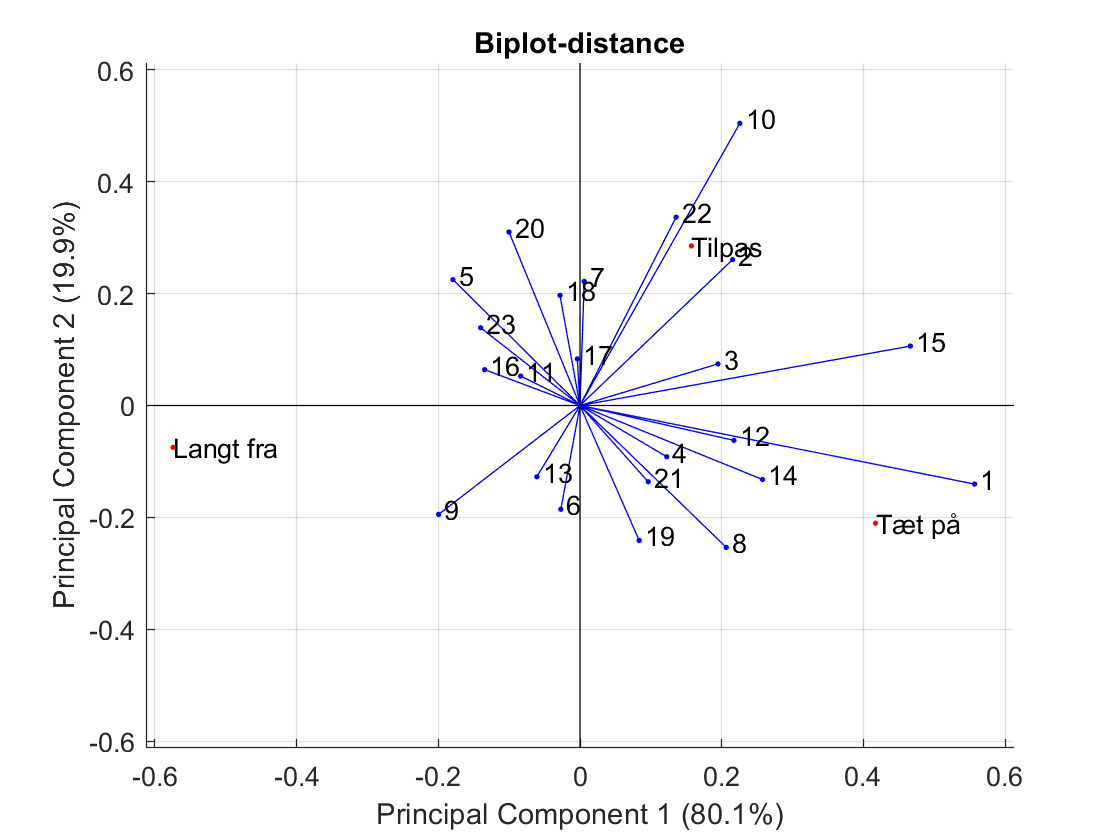
\includegraphics[width=\textwidth]{Figure/DatabehandlingSkalaer/PCAfigures/Distance-Biplot.png}
\caption{\textit{Bi}-plot med både \textit{loadings} (angivet med blå) og \textit{scores} (angivet med rød) fremgår i forhold til robottens afstand.}
\label{fig:Distance-Biplot}
\end{figure}
\noindent
%
Hver \textit{loading} angiver hvor meget variation hver parameter bidrager med på den specifikke PC. I \autoref{tab:LoadingsHoejde} fremgår samtlige \textit{loadings} for hver parameter til hver PC.



\begin{table}[H]
\centering
\begin{tabular}{c|c|c}
    & PC1 (80.1\%)    & PC2 (19.9\%)    \\ \hline
SQ1  & \textbf{0.5567} & -0.1405         \\ \hline
SQ2  & 0.2152          & 0.2608          \\ \hline
SQ3  & 0.1945          & 0.0744          \\ \hline
SQ4  & 0.1224          & -0.0917         \\ \hline
SQ5  & -0.1793         & 0.2251          \\ \hline
SQ6  & -0.0271         & -0.1856         \\ \hline
SQ7  & 0.0059          & 0.2217          \\ \hline
SQ8  & 0.2064          & -0.2537         \\ \hline
SQ9  & -0.1995         & -0.1946         \\ \hline
SQ10 & 0.2255          & \textbf{0.5045} \\ \hline
SQ11 & -0.0838         & 0.0526          \\ \hline
SQ12 & 0.2171          & -0.0623         \\ \hline
SQ13 & -0.0609         & -0.1274         \\ \hline
SQ14 & 0.2575          & -0.1323         \\ \hline
SQ15 & 0.4661          & 0.1062          \\ \hline
SQ16 & -0.1346         & 0.0641          \\ \hline
SQ17 & -0.0038         & 0.0834          \\ \hline
SQ18 & -0.0283         & 0.1969          \\ \hline
SQ19 & 0.0834          & -0.2412         \\ \hline
SQ20 & -0.1002         & 0.3102          \\ \hline
SQ21 & 0.0962          & -0.1363         \\ \hline
SQ22 & 0.1356          & 0.3367          \\ \hline
SQ23 & -0.1403         & 0.1390         
\end{tabular}
\caption{Oversigt over \textit{loadings} til de to PCs, for hver PC fremhæves den mest betydende parameter. \textit{SQ} angiver skala spørgsmålet.}
\label{tab:LoadingsAfstand}
\end{table}
\noindent
%
Tages der derimod udgangspunkt i et tredimensionelt \textit{Bi}-plot, jævnfør \autoref{fig:RHeight-3D}, fremgår det, at de to højder: 129 cm og 140 cm adskiller sig en del i den tredje dimension. Derudover tyder det på, at SQ6, som vedrører testpersonernes oplevelse af robottens hastighed, samt SQ10, som vedrører hvor tryg testpersonen følte sig ved robotten, er de to parametre, som har størst indflydelse på PC3. 

Derudover elimineres nogen af de førnævnte korrelationer mellem parametrene, når de præsenteres i det tredimensionelle plot, gengivet på \autoref{fig:RHeight-3D}. Dette gælder blandt andet SQ2 og SQ4, som ikke længere ligger oven på hinanden.   
%
\begin{figure}[H]
\centering
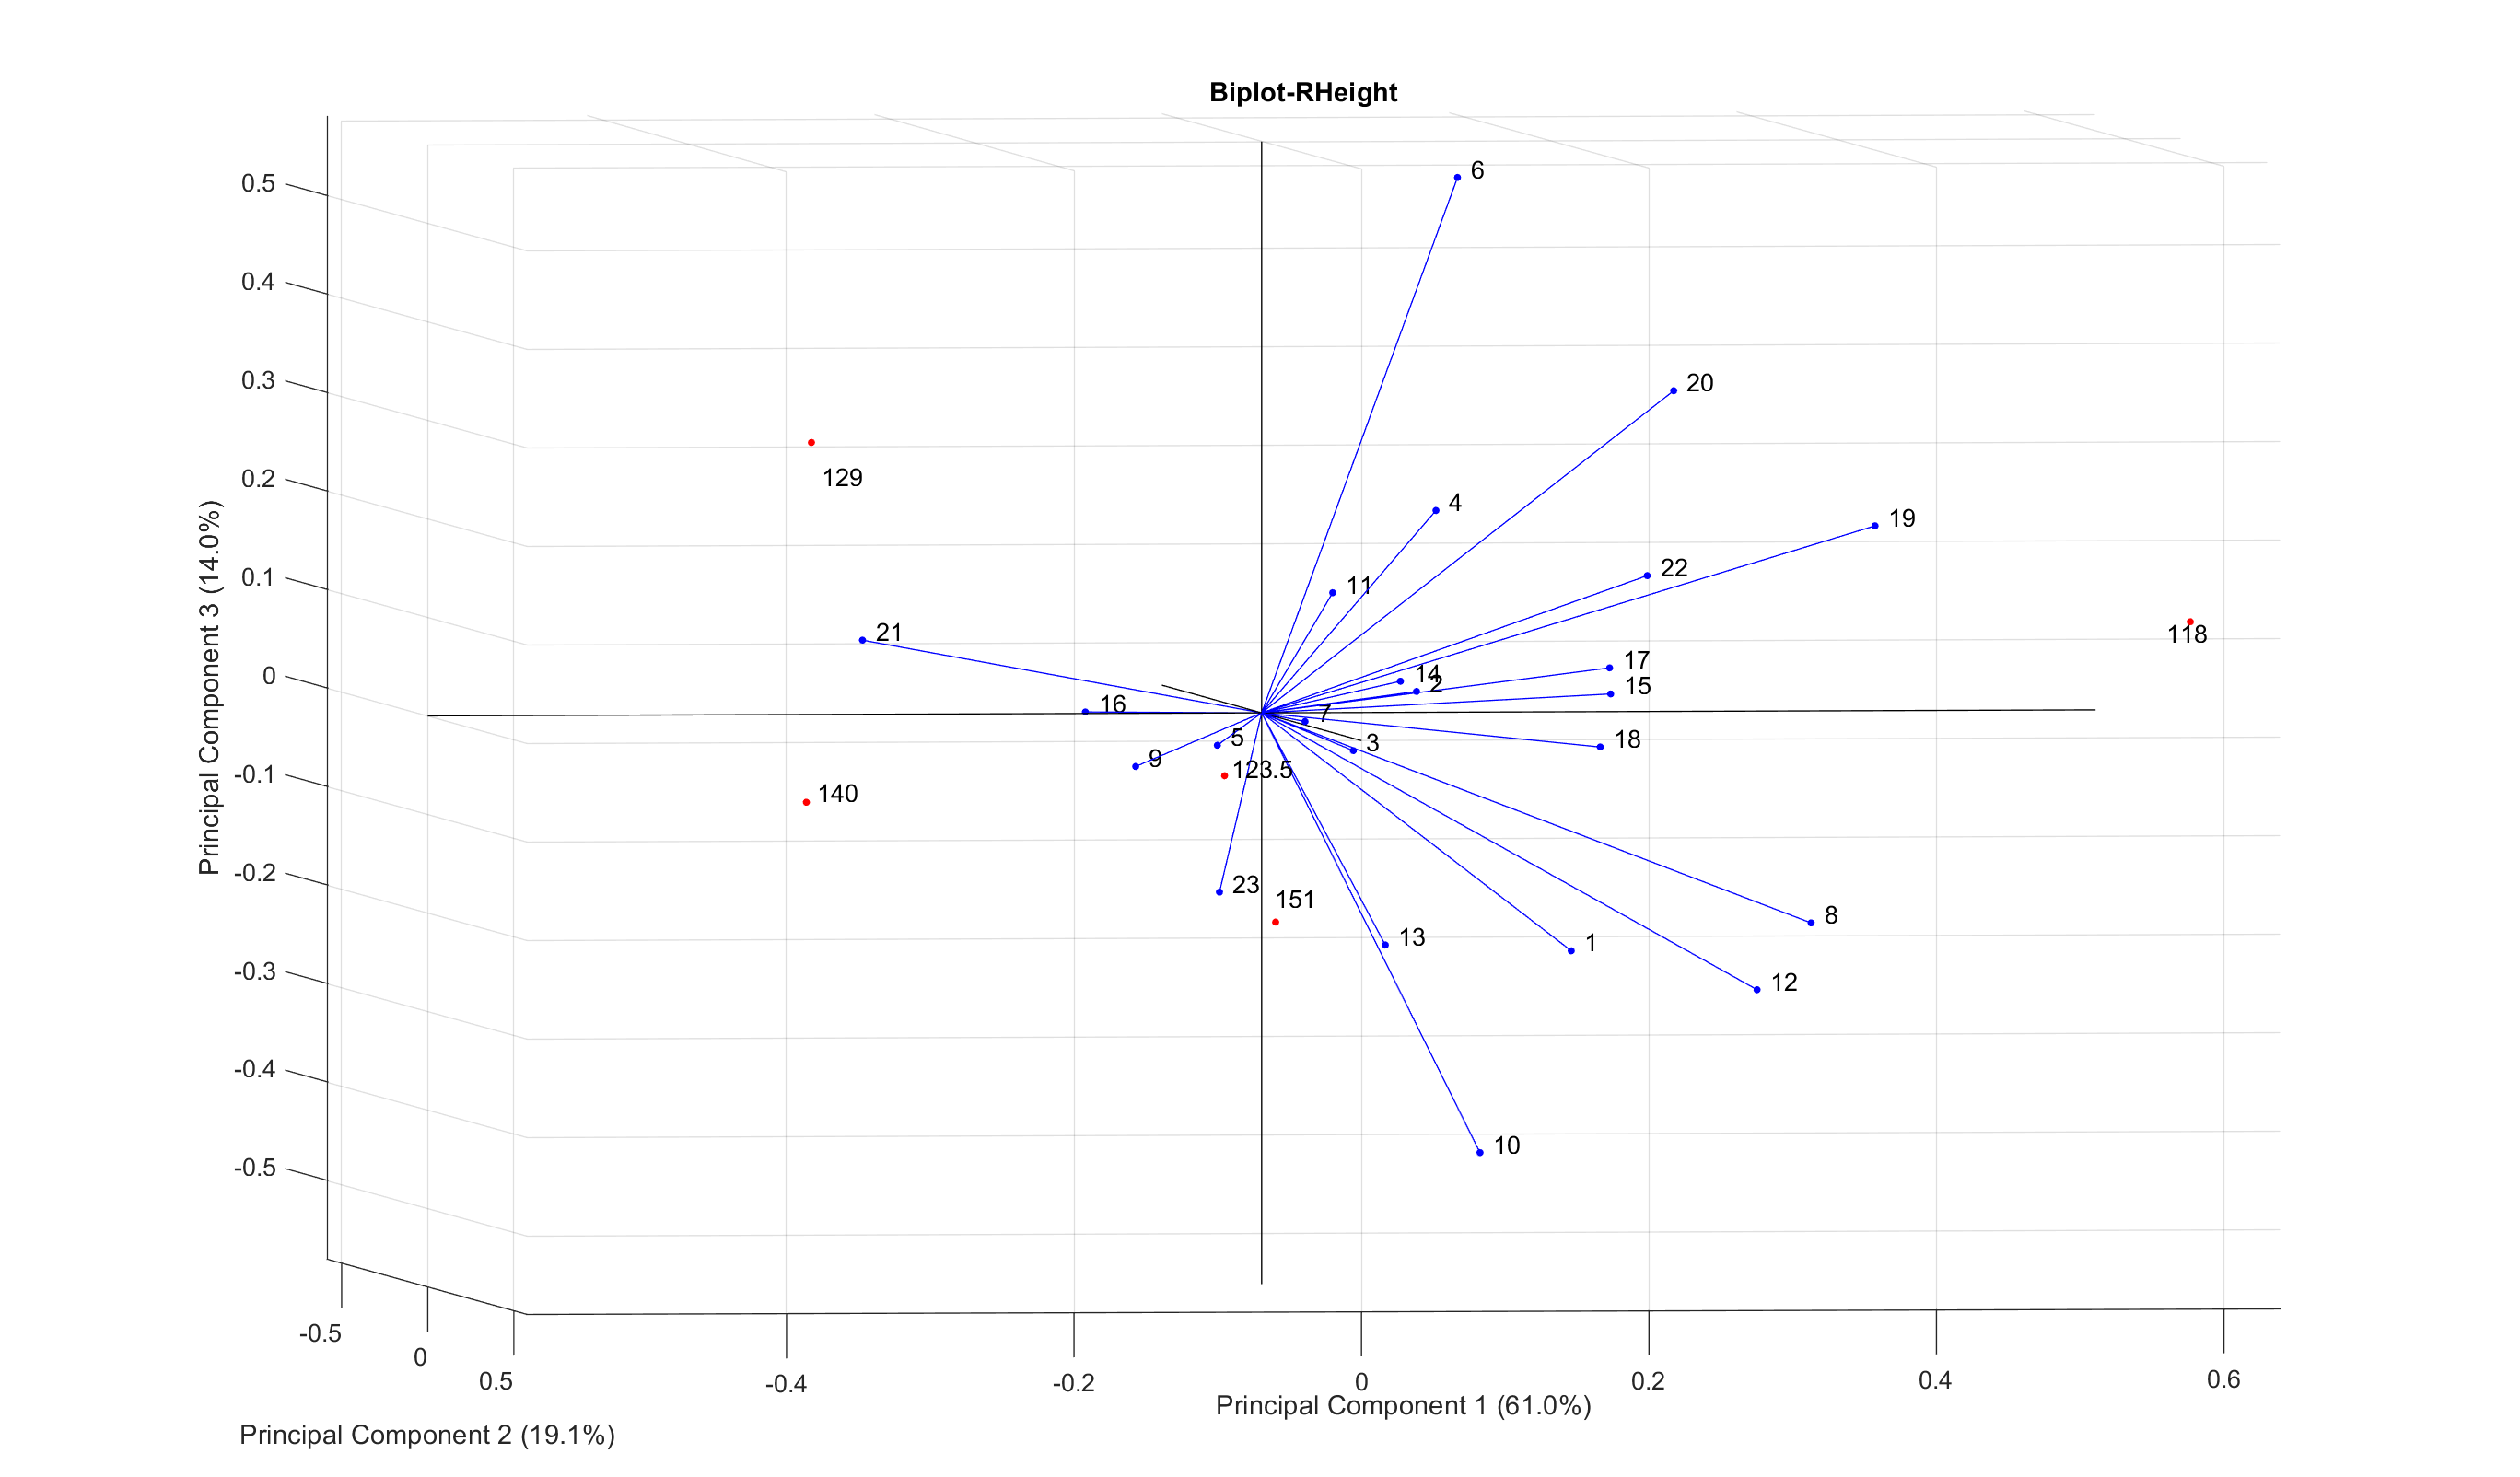
\includegraphics[width=\textwidth]{Figure/DatabehandlingSkalaer/PCAfigures/RHeight-3D.png}
\caption{3D \textit{Bi}-plot med både \textit{loadings} (angivet med blå) og \textit{scores} (angivet med rød) fremgår i forhold til robottens højde.}
\label{fig:RHeight-3D}
\end{figure}
%

\subsection{Tendenser i forhold til robottens højde}
\label{DatabehandlingRHeightTendenser}
%
